\documentclass[../main.tex]{subfiles}

\begin{document}

\problem{1}

\textit{Note: All calculations performed in Python using custom module designed to analyze isentropic flow and normal shocks. See appendix \ref{Problem1Python} and https://github.com/ejburke73/py-compressible-flow.}

\problempart{a} 

Plot the vehicle's freestream Mach number \(M_\infty\) versus flight time \(t\) using realistic temperature values.
Plot the vehicle's freestream Mach number \(M_\infty\) versus flight time \(t\) using constant room temperature (\(T=298\,\unit{\kelvin}\)).
Plot the absolute magnitude of the difference in calculated \(M_\infty\) versus flight time \(t\) using both approaches.
Make your case whether or not to use accurate values for the local air temperature.

\givens{}
Vehicle trajectory, accurate air properties throughout duration of flight at all altitudes.
Constant room temperature, \(T=298\,\unit{\kelvin}\).

\assumptions{}
Air can be treated as an ideal gas with constant specific heats throughout the entire trajectory (i.e., CPG).
Isentropic flow.
\(\gamma_{air} = 1.4\). 
\(R_{air} = 287 \, \unit{\joule/\kilogram\cdot\kelvin}\). 
The flow around the vehicle can be treated as inviscid.

\solution{}
Using the definition of the speed of sound, \(a=\sqrt{\gamma R T}\), vehicle freestream velocity, \(u\), and accurate air temperatures at all altitudes, \(M_{\infty,i}\) is easily calculated at all \(t=i\) in the trajectory.

\[
    M_{\infty,i} = \frac{u_i}{\sqrt{\gamma R T_i}}  
\]

The same relationship can be used with a constant \(T=298\,\unit{\kelvin}\) to calculate \(M_{\infty,i}\) at all \(t=i\) in the trajectory.

\[
    M_{\infty,i} = \frac{u_i}{\sqrt{\gamma R \cdot 298 \, \unit{\kelvin}}}  
\]

Figure \ref{Mach_correct} shows the freestream Mach versus time, calculated using accurate atmospheric air temperatures.

\begin{figure}[h]
    \centering
    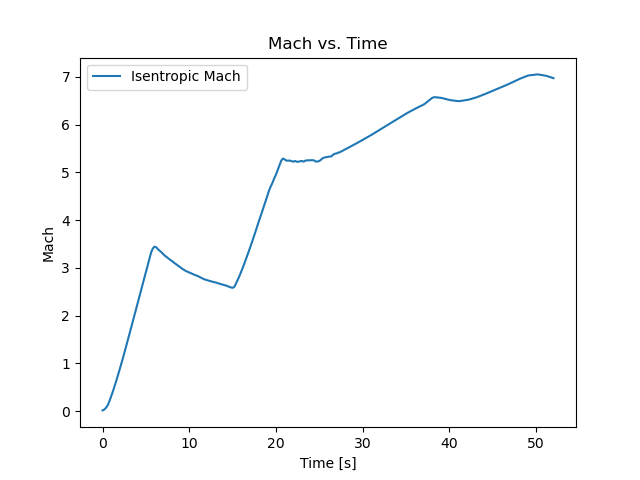
\includegraphics[scale=.7]{../../images/problem_1/Mach_correct_vs_Time.png}
    \caption{Mach vs. Time using accurate air temperature values}
    \label{Mach_correct}
\end{figure}

Figure \ref{Mach_298} shows the freestream Mach versus time, calculated using a constant air temperature of \(T=298\,\unit{\kelvin}\).

\begin{figure}[h]
    \centering
    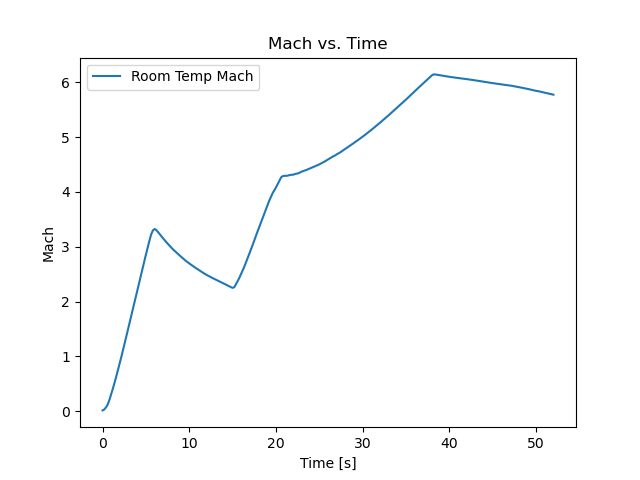
\includegraphics[scale=.7]{../../images/problem_1/Mach_298_vs_Time.png}
    \caption{Mach vs. Time using constant room temperature air}
    \label{Mach_298}
\end{figure}

Figure \ref{Mach} shows both calculated Mach histories including the abosolute error magnitude.

\begin{figure}[h]
    \centering
    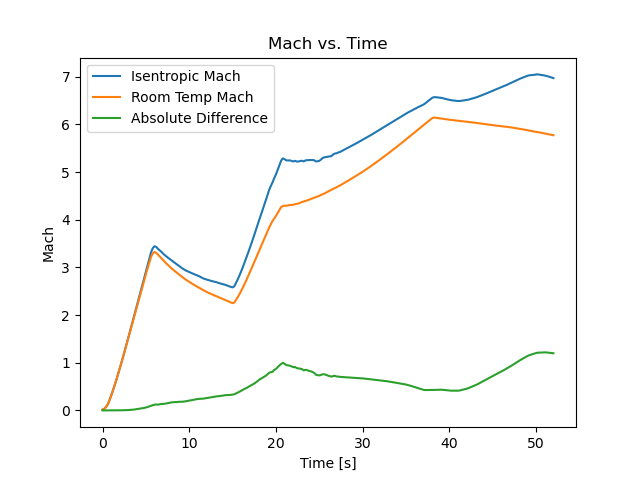
\includegraphics[scale=.7]{../../images/problem_1/Mach_vs_Time.png}
    \caption{Mach vs. Time comparison with absolute error magnitude}
    \label{Mach}
\end{figure}

Figure \ref{Mach_error} shows the absolute \% error between both methods of calculating Mach number.

\begin{figure}[h]
    \centering
    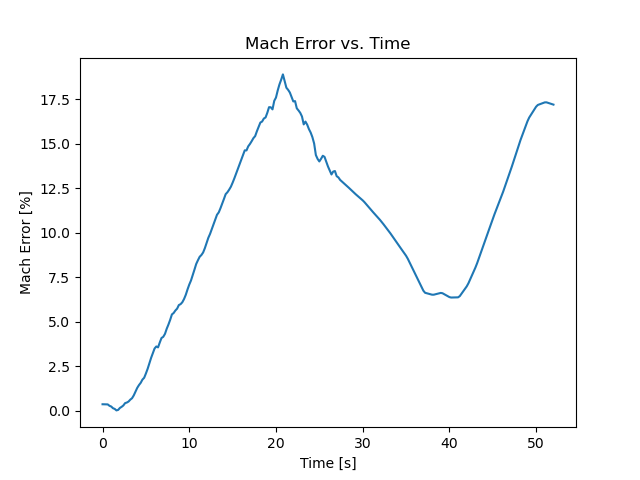
\includegraphics[scale=.7]{../../images/problem_1/Mach_Error_vs_Time.png}
    \caption{Absolute \% Mach error vs. Time}
    \label{Mach_error}
\end{figure}

\discussion{}

Using a constant room temperature value for air throughout all points of the trajectory would induce dramatic amounts of error to any subsequent calculations relevant to the experiments present on the vehicle.
Examining figure \ref{Mach_error}, we see up to 17.5 \% error between the methods of Mach calculation, corresponding to over an entire Mach number of difference at \(t=20\,\unit{\s}\).
There is no reason to use constant room temperature values when atmospheric conditions are so easily obtained and the difference in calculation method is nonexistent. 
To obtain \textbf{any} amount of accuracy, we must use accurate atmospheric conditions.

\clearpage

\problempart{b} 

Prove that use of compressible-flow equations is more appropriate than use of Bernoulli for analyzing the vehicle trajectory.
Provide a plot of \(\rho_\infty/\rho_0\) versus time and identify the first point in time at which flow is considered compressible.
Provide a plot of \(p_0\) versus time caculated both using isentropic relations and Bernoulli's equation.
Are there times where the total pressure values agree?
If so, when and why?
Mathematically prove that for \(M<<1\) the isentropic equation for \(p_0/p_\infty\) becomes exactly the Bernoulli equation.

\givens{}
Flight data from trajectory.

\assumptions{}
Air can be treated as an ideal gas with constant specific heats throughout the entire trajectory (i.e., CPG).
Isentropic flow.
\(\gamma_{air} = 1.4\). 
\(R_{air} = 287 \, \unit{\joule/\kilogram\cdot\kelvin}\). 
The flow around the vehicle can be treated as inviscid.

\solution{}

The isentropic flow relation for total-to-static density is given by:

\[
    \frac{\rho_0}{\rho_\infty} = \left({1 + \frac{\gamma-1}{2} M_\infty^2}\right) ^ {\frac{1}{\gamma-1}}   
\]

Obtaining \(\rho_\infty/\rho_0\) involves a simple reciprocal.
Figure \ref{rho_rho_t_time} shows the time history of the static to total density ratio, \(\rho_\infty/\rho_0\) versus time.
There is a rapid reduction in the ratio indicating that compressibility comes into play quickly. 
Figure \ref{rho_rho_t_vs_Mach} shows the relationship between the density ratio and Mach number.
The freestream density has been reduced by ~25\% by the time the sonic condition is reached.
Figure \ref{rho_rho_t_vs_Mach_marked} compares the density ratio and Mach number both as a function of time, highlighting the exact point in time and Mach number where the fluid's density has changed by 5\%, our accepted definition of compressibility.
The marked points indicate that at \(M_\infty = 0.31\) and \(t=1 \, \unit{\s}\), there is a 5\% reduction in static density relative to total density.
The flow becomes compressible almost immediately in the trajectory, and we must use appropriate compressible relations to account for that through the entirety of the time history.

\begin{figure}[h!]
    \centering
    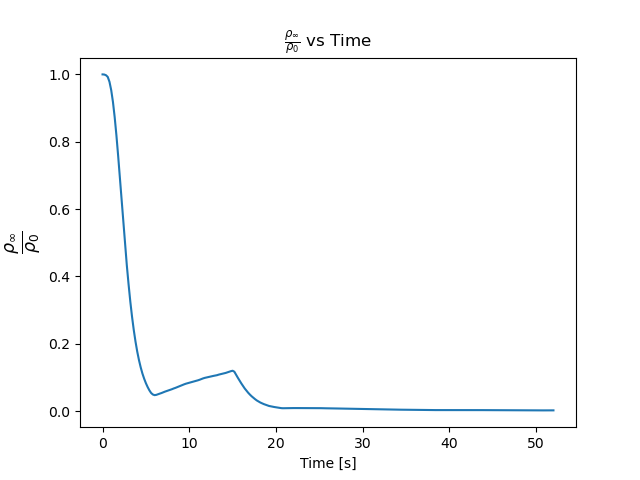
\includegraphics[scale=.7]{../../images/problem_1/rho_rho_t_vs_Time.png}
    \caption{Static to total density ratio vs. time}
    \label{rho_rho_t_time}
\end{figure}

\begin{figure}[h!]
    \centering
    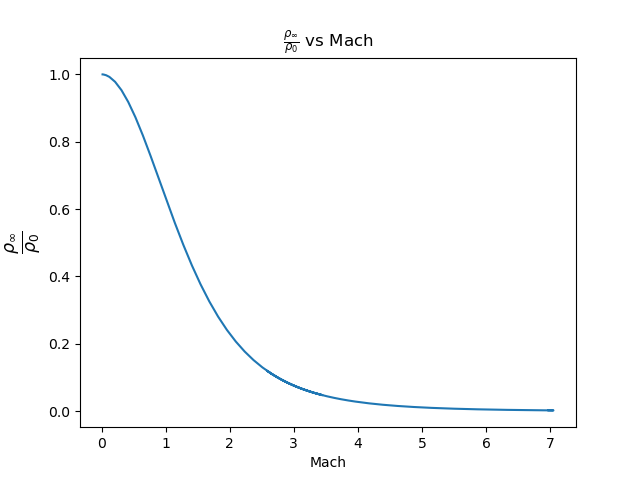
\includegraphics[scale=.7]{../../images/problem_1/rho_rho_t_vs_Mach.png}
    \caption{Static to total density ratio vs. Mach}
    \label{rho_rho_t_vs_Mach}
\end{figure}

\begin{figure}[h!]
    \centering
    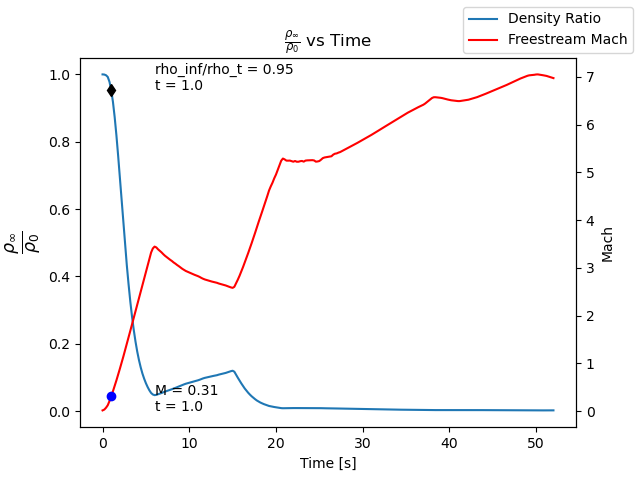
\includegraphics[scale=.7]{../../images/problem_1/rho_rho_t_and_Mach_vs_Time_marked.png}
    \caption{Density ratio and Mach vs.s time}
    \label{rho_rho_t_vs_Mach_marked}
\end{figure}

The isentropic relation for total pressure is given by the following:

\[
    p_0 = p_\infty {\left({1 + \frac{\gamma-1}{2}M_\infty^2}\right)}^{\frac{\gamma}{\gamma-1}}  
\]

The incompressible relation, known as Bernoulli's equation, is given by the following:

\[
    p_0 = p_\infty + \frac{1}{2} \rho_\infty u^2
\]

This equation does not take compressibility into account and is not accurate for flows above \(M \approx 0.3\).
To prove this, figure \ref{Pt_v_t} shows a comparison of the total pressure calculated using both methods. 
There is a substantial difference in calculated total pressure during the trajectory.
The two equations do yield the same values at the beginning of the trajectory when the Mach number is sufficiently small so that the flow is essentially incompressible.
At the end of the trajectory, the values are also similar because of the very small freestream density and atmospheric pressure at very high altitudes.

\begin{figure}[h!]
    \centering
    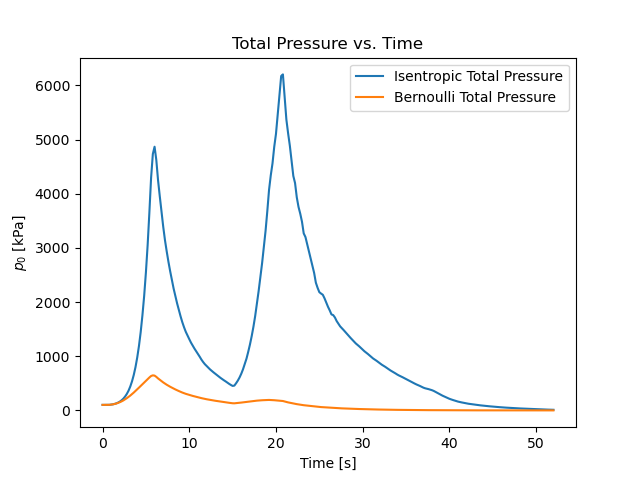
\includegraphics[scale=.7]{../../images/problem_1/Pt_vs_Time_Isen_Bernoulli.png}
    \caption{Total pressure vs. time using isentropic relations and Bernoulli}
    \label{Pt_v_t}
\end{figure}

For proof that the isentropic equation and Bernoulli's equation are identical for small Mach numbers (\(M<<1\)), we begin by noting the following binomial expansion valid for \(x<<1\).

\[
    \left({1 + x}\right)^\alpha \approx 1 + \alpha x  
\]

The isentropic relationship for pressure ratio:

\[
    \frac{p_0}{p_\infty} = {\left({1 + \frac{\gamma-1}{2}M_\infty^2}\right)} ^ {\frac{\gamma}{\gamma-1}}  
\]

Using the binomial expansion on the above relation:

\[
    \frac{p_0}{p_\infty} = 1 + \left({\frac{\gamma-1}{2}M_\infty^2}\right) \left({\frac{\gamma}{\gamma-1}}\right)
\]

\[
    \frac{p_0}{p_\infty} = 1 + \left({\frac{\gamma}{2}M_\infty^2}\right) 
\]

\[
    \frac{p_0}{p_\infty} = 1 + \left({\frac{\gamma}{2}}\right)\left({{\frac{u_\infty}{a}}}\right)^2 
\]

\[
    \frac{p_0}{p_\infty} = 1 + \left({\frac{\gamma}{2}}\right)\left({{\frac{u_\infty^2}{\gamma R T_\infty}}}\right) 
\]

\[
    \frac{p_0}{p_\infty} = 1 + \frac{u^2}{2RT_\infty}
\]

\[
    \frac{p_0}{p_\infty} = 1 + \frac{\rho_\infty u^2}{2p_\infty}
\]

We now arrive at exactly Bernoulli's equation for incompressible flow:

\[
    \boxed{
    p_0 = p_\infty + \frac{1}{2} \rho_\infty u^2
    }
\]

\discussion{}
Through several methods, we have shown that the compressible flow equations are critical for use analysis of a high speed vehicle.
Compressibility effects begin very early in the flight (\(t=1\,\unit{\s}\)) and there are large amounts of error shown when not using the compressible equations for total pressure.
At low Mach numbers, we have shown that the isentropic relation collapses into the Bernoulli equation exactly.

\clearpage

\problempart{c}
Find a data point in the trajectory where both flight \(M_\infty\) and \(u_\infty\) exactly match the possible tunnel \(M_\infty\) and \(u_\infty\).
Indicate the flight time \(t\).
What are the flight \(M_\infty\) and \(u_\infty\) at \(t\)?
Assuming isentropic flow, what temperature do the tunnel's heated blankets need to be set to to achieve the correct stagnation temperature, \(T_0\)?
Does this seem like a reasonable value of \(T_0\) to achieve?
Is it possible to match both \(M_\infty\) and \(u_\infty\) simultaneously this facility?
If not, what other options can you think of?
Assuming you could achieve the appropriate \(T_0\), what would the freestream temperature in the throat of the nozzle be?

\givens{}
Flight data from trajectory.

\assumptions{}
Air can be treated as an ideal gas with constant specific heats throughout the entire trajectory (i.e., CPG).
Isentropic flow.
\(\gamma_{air} = 1.4\). 
\(R_{air} = 287 \, \unit{\joule/\kilogram\cdot\kelvin}\). 
The flow around the vehicle can be treated as inviscid.

\solution{}

From the trajectory data, with a target \(M_\infty\) of 6, the following closest point was identified:

\begin{align*}
    t &= 33 \, \unit{\s}\\
    M_\infty &= 6.007 \approx 6\\
    u_\infty &= 1868.7 \, \unit{\meter/\s}\\
    T_\infty &= 240.86 \, \unit{\kelvin}
\end{align*}

The total temperature at this condition is given by the following isentropic relation:

\[
    T_0 = T_\infty \left[{1 + \frac{\gamma-1}{2}M_\infty^2}\right] = 1979.1 \, \unit{\kelvin}
\] 

This value for total temperature seems excessively high and not achievable with heated blankets in a facility. 
Because we have no realistic way of heating the reservoir flow to achieve this total temperature, it is not possible to achieve both \(M_\infty\) and \(u_\infty\) in the tunnel.
An alternative method would be to use a smaller model with the same Mach number and Reynolds number and accept that there will be an enthalpy difference.

Assuming that this total temperature value was realistic, the freestream temperature in the nozzle throat, \(T^*\), is given by the isentropic temperature relation at the sonic condition, \(M=1\).

\[
    T^* = \frac{T_0}{\left[{1 + \frac{\gamma-1}{2}}\right]} = 1649.2 \, \unit{\kelvin}
\] 

\discussion{}

Although there is a flight condition with a \(M_\infty\) that the tunnel can achieve, it is not feasible to use heating blankets to achieve the requisite total temperature value needed to match \(u_\infty\) and flight enthalpy. 

\clearpage

\problempart{d}
Now that you have indicated to your boss/advisor that you have matching \(M_\infty\) and \(u_\infty\) conditions they think you should measure the same surface temperature on the model. 
Is this true? 
Explain yourself to them.
You may assume that the vehicle was the same size and at the same Reynolds number here.

\givens{}
The tunnel can achieve flight \(M_\infty\) and \(u_\infty\).

\assumptions{}
Assume the tunnel can achieve the correct total temperature value (proven false in previous section).
Air can be treated as an ideal gas with constant specific heats throughout the entire trajectory (i.e., CPG).
Isentropic flow.
\(\gamma_{air} = 1.4\). 
\(R_{air} = 287 \, \unit{\joule/\kilogram\cdot\kelvin}\). 
The flow around the vehicle can be treated as inviscid.
Vehicle model is at the same scale as the flight article.
The tunnel can also match flight Reynolds number.

\solution{}

Assuming that the tunnel can achieve the correct stagnation temperature for the flow, a \(M_\infty = 6\) tunnel condition, and properly match Reynolds number, the surface heating of an identically sized model should be the same as the flight article.

If we assume that \(M_\infty\) and \(u_\infty\) are matched, we observe the following:

\[
    M_{flight} = M_{tunnel}
\]

\[
    \frac{u_{flight}}{a_{flight}} = \frac{u_{tunnel}}{a_{tunnel}}
\]

\[
    a_{flight} = a_{tunnel}
\]

\[
    \sqrt{\gamma R T_{flight}} = \sqrt{\gamma R T_{tunnel}}
\]

\[
    \boxed{
     T_{flight} = T_{tunnel}
    }
\]

We observe that matching \(M_\infty\) and \(u_\infty\) implies that static temperatures are identical.
Now, we examine Reynolds number:

\[
    Re = \frac{\rho u L}{\mu}
\]

We have assumed that Reynolds number is matched exactly and the tunnel article is the same size as the flight vehicle.

\[
    Re_{flight} = Re_{tunnel}
\]

\[
    \left({\frac{\rho u L}{\mu}}\right)_{flight} = \left({\frac{\rho u L}{\mu}}\right)_{tunnel}
\]

Viscosity, \(\mu\), is only a function of temperature.
Therefore, we know that the viscosity on both sides is equal and can be removed.
We also know that the length scale of both vehicles is the same, as is the freestream velocity.

\[
    \mu = \mu(T)
\]

This results in the following observation: the densities are identical. 

\[
    \boxed{
    \rho_{flight} = \rho_{tunnel}
    }
\]

Because we have assumed that air is an ideal gas and we have determined that both \(T\) and \(\rho\) are identical, we know that \(p\) must also match and have proven that the air moving through the tunnel is identical to the air experienced at Mach 6 during the trajectory.
With all of the above results, there is no possible way for the aeroheating, and therefore surface temperature, to be different assuming the models have identical surface material properties.

\discussion{}

Assuming that the Mach 6 tunnel can match freestream velocity and Reynolds number for a tunnel model identical to the flight article, the tunnel model will experience the same surface temperatures as the flight vehicle.
This is not truly possible due to limitations in reservoir heating.

\end{document}